%% This is an example first chapter.  You should put chapter/appendix that you
%% write into a separate file, and add a line \include{yourfilename} to
%% main.tex, where `yourfilename.tex' is the name of the chapter/appendix file.
%% You can process specific files by typing their names in at the 
%% \files=
%% prompt when you run the file main.tex through LaTeX.
\chapter{Teoretický rozbor}
Před vlastním návrhem a realizací je nezbytně nutné být seznámen alespoň se základní teorií použitých technologií a postupů. Bez této znalosti by se jednalo pouze o útržky textu a nebylo by možno zacházet do řešení komplexnější problematiky a kladení možných dalších témat pro následující výzkum a posun technologie.

\section{3D tisk a materiály}
3D tisk je na rozdíl od jiných technologií aditivní proces. Jedná se tedy o postupné přidávání základního materiálu v diskrétních krocích (vrstvách).
Technologií existuje několik a s postupným rozšiřováním možností aplikace jich stále přibývá. Pro řešení této práce byla vybrána technologie FDM vzhledem k jejímu masovému rozšíření, dostupnosti a nízkých nákladů. 

\subsection{Princip technologie FDM}
Fused deposition modeling, zkráceně FDM, případně FFF (Fused Filament Fabrication) je technologie 3D tisku využívající možnost opakovatelného přechodu mezi skupenstvími působením energie ve formě tepla termoplastických polymerních materiálů. Základní materiál ve formě filamentu (drátu) definovaného průměru, zpravidla 1.75\,mm, nebo 2.85\,mm, je vtlačován do předehřáte trysky silou $F$. Pokud teplota horké zóny trysky převyšuje teplotu skelného přechodu vtlačovaného materiálu dojde k dramatickému oslabení mezimolekulárních sil a vzniku viskózní kapaliny. Jelikož je průměr trysky velmi blízký průměru vtlačovaného filamentu, s vyjímkou jejího hrdla které je násobně menší, zpravidla 0.4\,mm, jediná možnost jak uvolnit vnitřní tlak je vytlačení kapaliny hrdlem. Jakmile teplota vytlačené kapaliny klesne pod teplotu skelného přechodu dojde k obnovení mezimolekulárních sil a materiál je opět pevnou látkou. Tento jev je obecně znám pod názvem extruze, zařízení .
Toto nám však nestačí pro vytvoření trojrozměrného objektu dle zadání. Je tedy třeba extrudér osadit na zařízení zajišťující pohyb v trojrozměrném prostoru.
Proces tisku pak probíhá pohybem extrudéru po předem definovaných trasách, zpravidla vždy v jedné vrstvě, a vytlačováním materiálu dle potřeby. Celý proces se poté opakuje dokud není dokončen zadaný objekt.
\begin{figure}[h]
\begin{center}
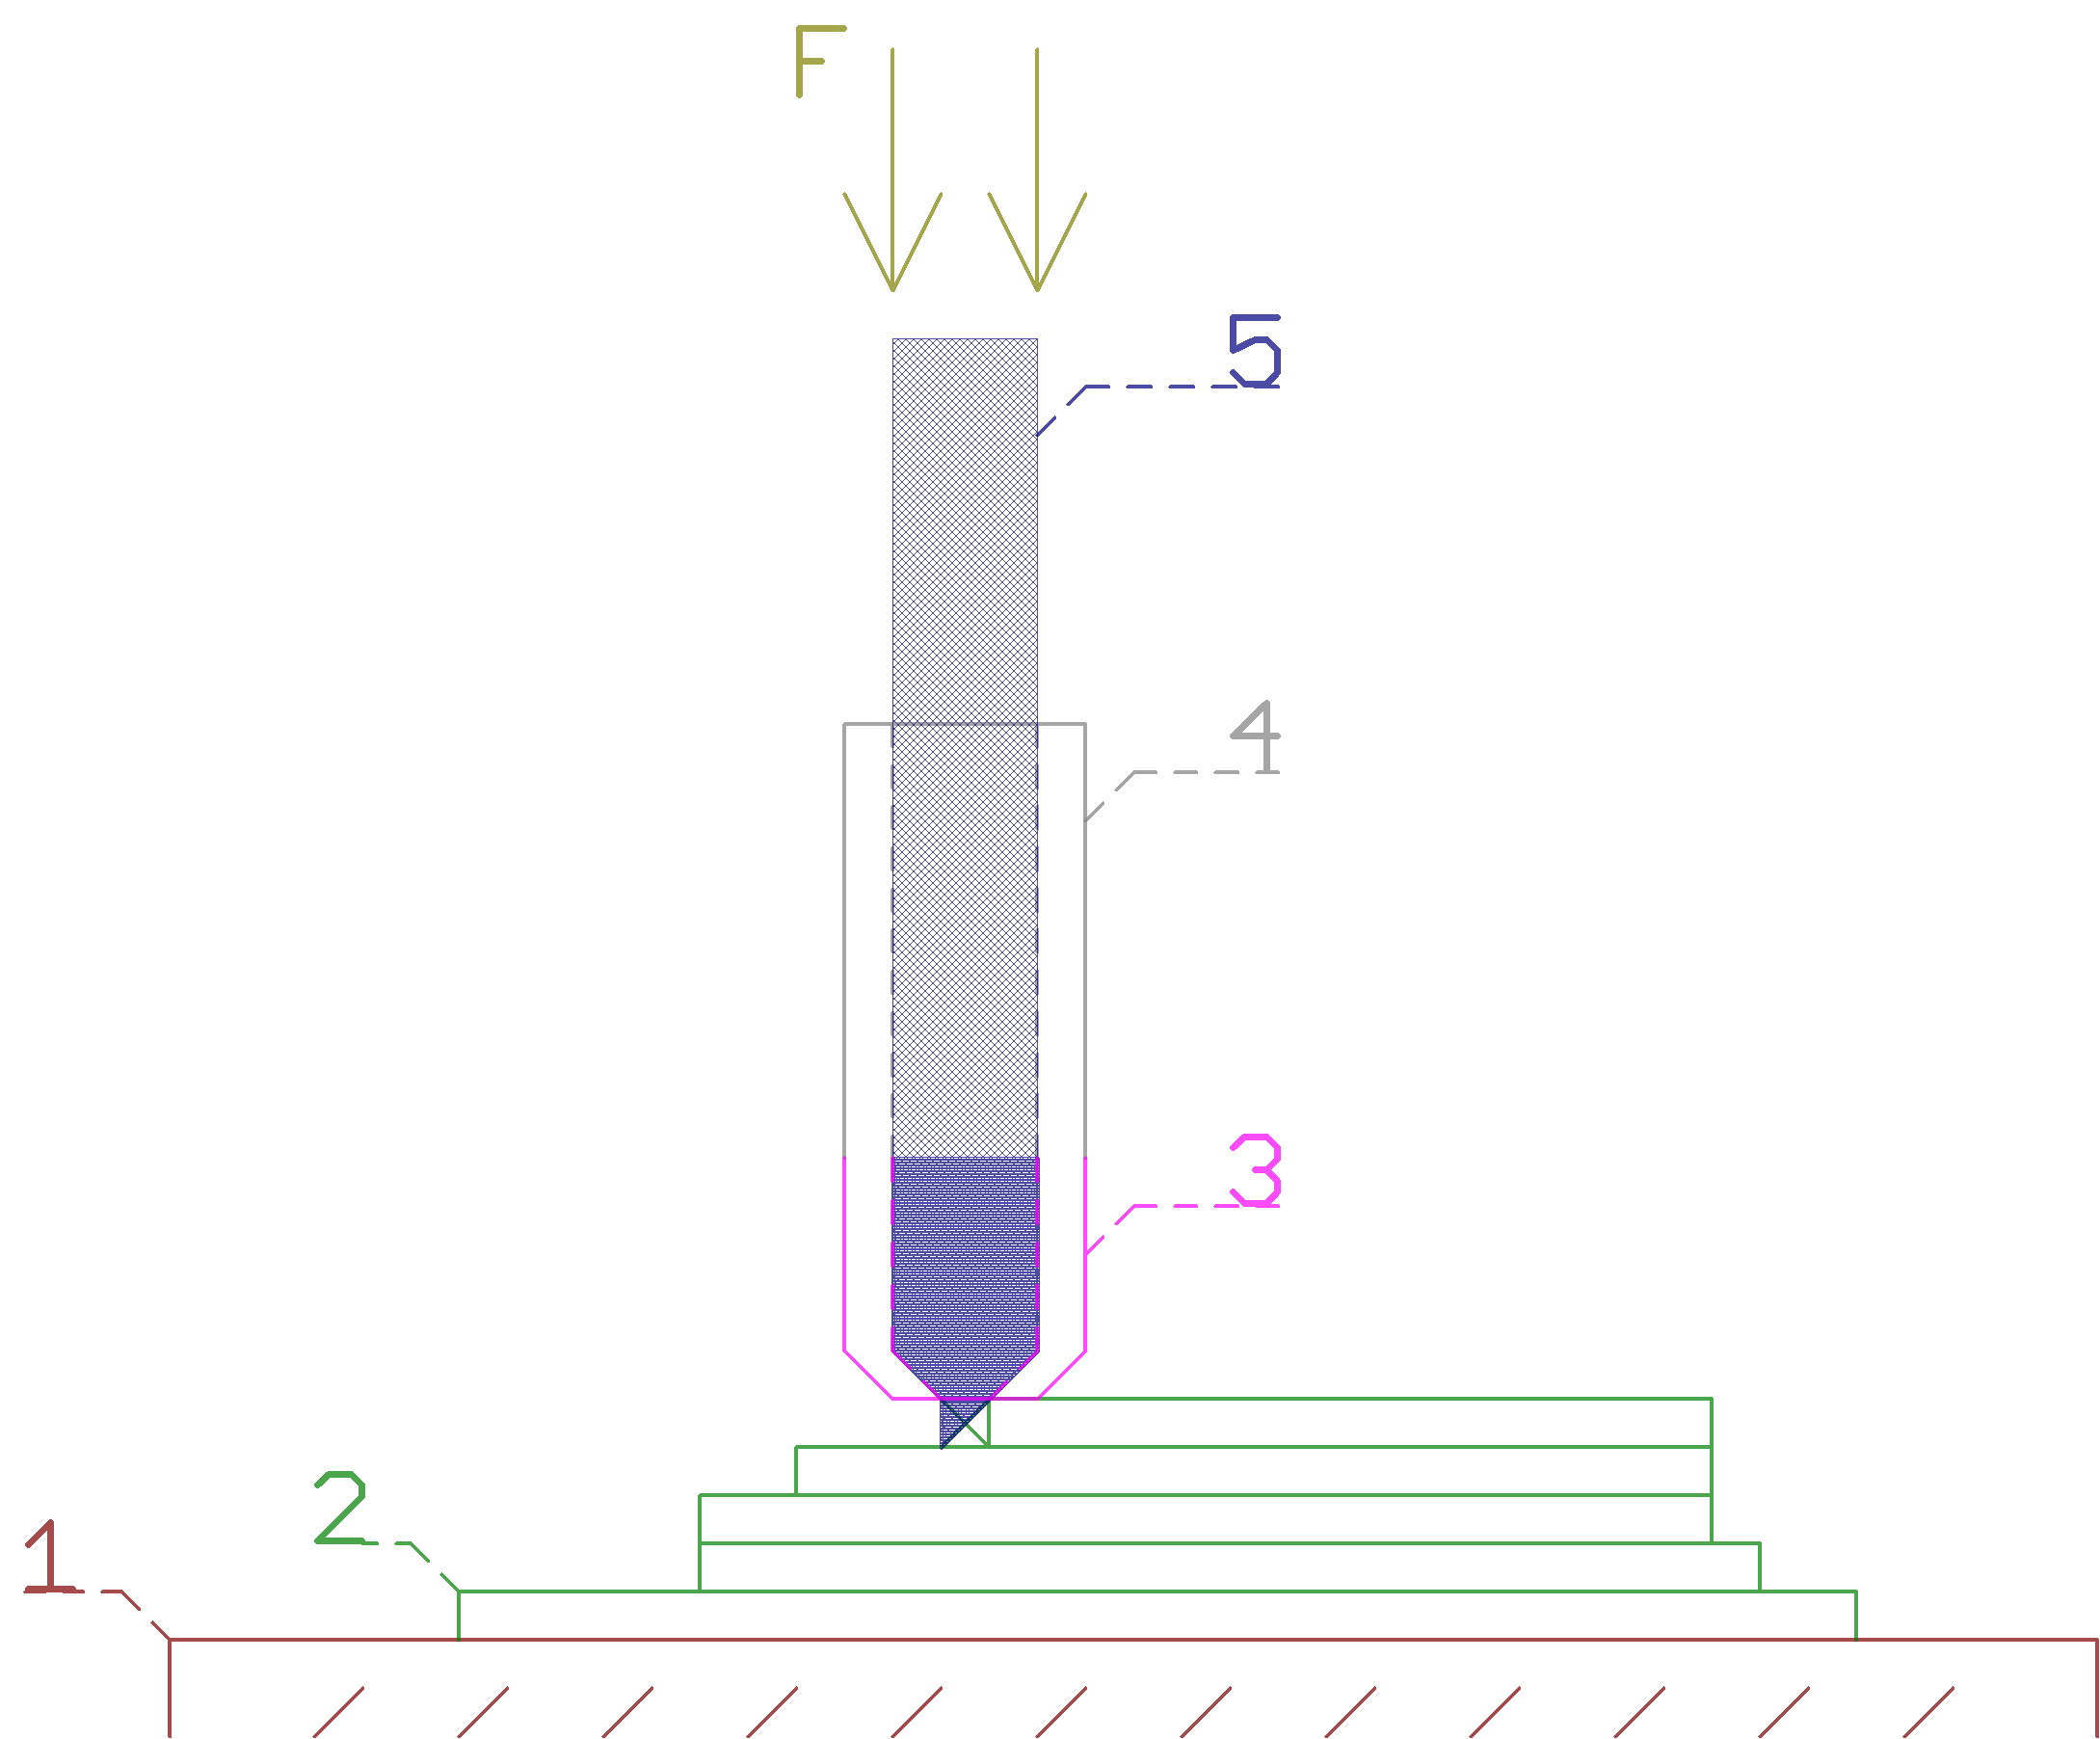
\includegraphics[width=9.5cm]{pics/fdm}
\caption{Princip technologie FDM. 1 - Tisková podložka, 2 - Již hotové vrstvy výsledného objektu, 3 - Horká zóna trysky, 4 - Tryska, 5 - Filament, F - Vtlačovací síla}
\end{center}
\end{figure}

\subsection{Vlastnosti technologie}


\subsection{Materiály využitelné pro vysokofrekvenční techniku}


\section{Trychtýřová anténa}
Trychtýřová anténa patří mezi základní anténní struktury využívané jak samostatně, tak ve formě ozařovačů reflektorových antén, či v kombinaci s anténní čočkou. Těchto struktur existuje několik druhů, v našem případě se ale zaměříme na pyramidální trychtýřovou anténu.
Tento typ antény byl zvolen zejména kvůli své jednoduchosti a požadavkům na technologii výroby.

\subsection{Základní princip}
\subsection{Vlastnosti struktury}


\section{Anténní čočka}

\subsection{Základní princip}
\subsection{Vlastnosti struktury}




\section{Extrakce dielektrických parametrů}